\newpage
\section{Problem 2: GEOMETRICAL MODIFICATION}\label{problem-2-geo-modify}
In this problem, please design several geometrical modification algorithms to meet the following requirements. Your results don’t have to be exactly the same as sample images, just try to make the effects.

\subsection{(a)}\label{2_a}
Please design an algorithm to make \textbf{sample3.jpg} become \textbf{sample4.jpg}. Output the result as \textbf{result6.jpg}. Please describe your method and implementation details clearly. (hint: you may perform rotation, scaling, translation, etc.)

Original image \nameref{sample3} for question \nameref{2_a}.
\begin{figure}
    \centering
    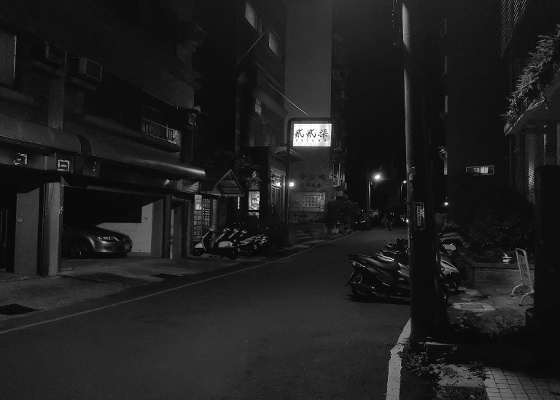
\includegraphics[width=0.7\textwidth]{hw2_sample_images/sample3.jpg}
    \caption{\textbf{sample3.jpg}}
    \label{sample3}
\end{figure}

\paragraph{Motivation}
I think we could observe \nameref{prob2a_reference_line} and get:
\begin{itemize}
    \item Rotate $78^{\circ}$.
    \item Scale up $150$\%.
    \item Shift from current to $(-200, 150)$.
\end{itemize}
 
\begin{figure}
    \centering
    \includegraphics[width=0.5\textwidth]{hw2_sample_images/prob2a_reference_line.png}
    \caption{Reference line of problem 2 (a)}
    \label{prob2a_reference_line}
\end{figure}

\paragraph{Approach}
We could follow the structure of \textbf{generalized linear geometrical transformation}, and use \textbf{backward treatment} in \textit{Lec 3 page 56 \& 50}.
\begin{enumerate}
    \item Design the \textbf{translation, scaling, rotation} matrix as operators in \textit{Lec 3 page 54}.
    \item Build operators $A^{-1}$, which is inverse of multiplication of above operations $A$.
    \item Build \textbf{grid map} of \textit{xy vectors}. \\
    Remember shift it to center by minus $(\frac{\mbox{width}}{2}, \frac{\mbox{height}}{2})$ of image size. \\
    As original point is the center of image.
    \item Get \textit{uv vectors} by applying inverse transform $A^{-1}$ on \textit{xy vectors}.
    \item Shift \textit{uv vectors} \& \textit{xy vectors} to original position by add $(\frac{\mbox{width}}{2}, \frac{\mbox{height}}{2})$.
    \item Get pixels within image boundaries. That means check whether \textit{uv vectors} are all in the image range.
    \item Create the blank canvas and draw from the original image on it. \\
    I use the \textbf{nearest neighbor interpolation} by rounding \textit{xy vectors} as well as \textit{uv vectors} into integer.
\end{enumerate}

\paragraph{Performance of results}
As former observation, I select rotate $78^{\circ}$, scale up $150$\% and
shift to $(-200, 150)$.

Result of problem 2(a): \nameref{result6}.
\begin{figure}
    \centering
    \includegraphics[width=0.7\textwidth]{hw2_sample_images/result6.jpg}
    \caption{\textbf{result6.jpg} of problem 2 (a)}
    \label{result6}
\end{figure}

\paragraph{Discussion}
I also try the \textbf{forward treatment}, and we could see some \alert{black grid} over the image \nameref{result6}.
\begin{figure}
    \centering
    \includegraphics[width=0.5\textwidth]{hw2_sample_images/tmp/result6_forward.jpg}
    \caption{\textbf{result6.jpg} problem 2 (a) by forward treatment}
    \label{result6_forward}
\end{figure}

\subsection{(b)}\label{2_b}
Imagine that there is a black hole in the center absorbing \textbf{sample5.jpg}. Please design a method to make \textbf{sample5.jpg} look like \textbf{sample6.jpg} as much as possible and save the output as \textbf{result7.jpg}.

Original image \nameref{sample5} for question \nameref{2_b}.
\begin{figure}
    \centering
    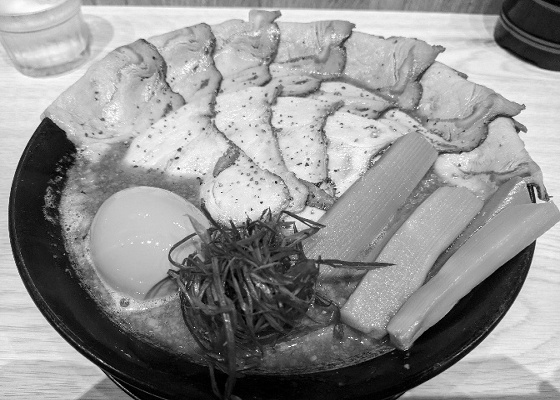
\includegraphics[width=0.7\textwidth]{hw2_sample_images/sample5.jpg}
    \caption{\textbf{sample5.jpg}}
    \label{sample5}
\end{figure}

\paragraph{Motivation}
After observing \nameref{prob2b_reference_line}, I feel maybe we could start from \textit{Polar coordinate system}. Because it seems the \textbf{twisted} of original image grid map.

\begin{figure}
    \centering
    \includegraphics[width=0.5\textwidth]{hw2_sample_images/prob2b_reference_line.png}
    \caption{Reference line of problem 2 (b)}
    \label{prob2b_reference_line}
\end{figure}

\paragraph{Approach}
Thanks to TAs and my friends explanation. I try this steps of \textit{blackhole}:
\begin{enumerate}
    \item Set up the parameters:
    \begin{itemize}
        \item \texttt{rotation\_radius}: radius of rotation from center.
        \item \texttt{twist\_scale}: The scale of twist.
        \item \texttt{hole\_radius}: the radius of holw. \\
        Note: it is a litter different from \texttt{rotation\_radius}, it affects \textbf{size of absorbing center}.
    \end{itemize}
    \item Calculate radius $r$ \& angle $\theta$ from center of image.
    \item Calculate \alert{absorbing scale} w.r.t radius and \texttt{rotation\_radius} with formula \\
    \(\mbox{absorb\_scale} = 0.4(1.0 - \frac{r}{\mbox{rotation\_radius}})^8\)
    \item We only change the \textbf{absorb scale} $>0$ as we could absorb the pixels to radius $=0$.
    \item Create the blank canvas and draw from the original image on it. \\
    I use the \textbf{nearest neighbor interpolation} by rounding \textit{xy vectors} as well as \textit{uv vectors} into integer. \\
    Note: A little difference here is we need to give \textbf{different scale} for \texttt{absorb\_scale}. So I go back to use \texttt{for loop} instead of matrix.
\end{enumerate}

\paragraph{Performance of results}
In the end, I select the following parameters as the last submission.
\begin{itemize}
    \item \texttt{rotation\_radius = 1000.0}
    \item \texttt{twist\_scale = 0.4}
    \item \texttt{hole\_radius = 100}
\end{itemize}

Result of problem 2(a): \nameref{result7}.
\begin{figure}
    \centering
    \includegraphics[width=0.7\textwidth]{hw2_sample_images/result7.jpg}
    \caption{\textbf{result7.jpg} of problem 2 (b)}
    \label{result7}
\end{figure}

\paragraph{Discussion}

The original idea is making a \textbf{vortex}. But we couldn't get the operators $A$ \& $A^{-1}$ at this time.
\begin{enumerate}
    \item Build \textbf{grid map} of \textit{xy vectors}. \\
    Remember shift it to center by minus $(\frac{\mbox{width}}{2}, \frac{\mbox{height}}{2})$ of image size. \\
    As original point is the center of image.
    \item Convert from \textit{Cartesian Coordinates} $(x, y)$ to \textit{Polar Coordinates} $(r, \theta)$ (radius and angle).
    \item Design \textbf{spiral transformation}, this is my \alert{main parts}: \\
    Let we inverse $(r, \theta)$ backward to $(\rho, \phi)$, given scalar $k$, s.t.
    \begin{itemize}
        \item $\phi = \theta + \frac{k}{r + \epsilon}$
        \item $\rho = r$
    \end{itemize}
    Where $\epsilon$ is a small number to prevent \texttt{divide by zero}.
    \item Get \textit{uv vectors} by converting from \textit{Polar Coordinates} $(\rho, \phi)$ to \textit{Cartesian Coordinates} $(u, v)$.
    \item Shift \textit{uv vectors} \& \textit{xy vectors} to original position by add $(\frac{\mbox{width}}{2}, \frac{\mbox{height}}{2})$.
    \item Get pixels within image boundaries. That means check whether \textit{uv vectors} are all in the image range.
    \item Create the blank canvas and draw from the original image on it. \\
    I use the \textbf{nearest neighbor interpolation} by rounding \textit{xy vectors} as well as \textit{uv vectors} into integer.
\end{enumerate}

It is really difficult to me that I can't figure out how to make \alert{absorbing effects}. My approach is creating the \alert{spiral}. But it keeps the center as \textit{vortex} not \textit{black hole}.

Maybe it is not a good way to conduct geometrical transformation on \textit{Polar coordinates}.

Result of problem 2(b): \nameref{result7_s}.
\begin{figure}
    \centering
    \includegraphics[width=0.7\textwidth]{hw2_sample_images/tmp/result7_spiral.jpg}
    \caption{\textbf{result7\_spiral.jpg} of problem 2 (b)}
    \label{result7_s}
\end{figure}